% Chapter 10: Comprehensive Review - Applied Time Series Analysis
% Harvard-quality academic presentation
% Bachelor program, Bucharest University of Economic Studies

\documentclass[9pt, aspectratio=169, t]{beamer}

% Ensure content fits on slides
\setbeamersize{text margin left=8mm, text margin right=8mm}

%=============================================================================
% THEME AND STYLE CONFIGURATION
%=============================================================================
\usetheme{Madrid}
\usecolortheme{seahorse}

% Professional Color Palette
\definecolor{MainBlue}{RGB}{26, 58, 110}
\definecolor{AccentBlue}{RGB}{42, 82, 140}
\definecolor{IDAred}{RGB}{220, 53, 69}
\definecolor{DarkGray}{RGB}{51, 51, 51}
\definecolor{MediumGray}{RGB}{128, 128, 128}
\definecolor{LightGray}{RGB}{248, 248, 248}
\definecolor{VeryLightGray}{RGB}{235, 235, 235}
\definecolor{Crimson}{RGB}{220, 53, 69}
\definecolor{Forest}{RGB}{46, 125, 50}
\definecolor{Amber}{RGB}{181, 133, 63}
\definecolor{Orange}{RGB}{230, 126, 34}
\definecolor{HarvardCrimson}{RGB}{165, 28, 48}

\setbeamercolor{palette primary}{bg=MainBlue, fg=white}
\setbeamercolor{palette secondary}{bg=MainBlue!85, fg=white}
\setbeamercolor{palette tertiary}{bg=MainBlue!70, fg=white}
\setbeamercolor{structure}{fg=MainBlue}
\setbeamercolor{title}{fg=MainBlue}
\setbeamercolor{frametitle}{fg=MainBlue, bg=white}
\setbeamercolor{block title}{bg=MainBlue, fg=white}
\setbeamercolor{block body}{bg=VeryLightGray, fg=DarkGray}
\setbeamercolor{block title alerted}{bg=Crimson, fg=white}
\setbeamercolor{block body alerted}{bg=Crimson!8, fg=DarkGray}
\setbeamercolor{block title example}{bg=Forest, fg=white}
\setbeamercolor{block body example}{bg=Forest!8, fg=DarkGray}
\setbeamercolor{item}{fg=MainBlue}

\setbeamertemplate{navigation symbols}{}

\setbeamertemplate{footline}{
    \leavevmode%
    \hbox{%
        \begin{beamercolorbox}[wd=.333333\paperwidth,ht=2.5ex,dp=1ex,center]{author in head/foot}%
            \usebeamerfont{author in head/foot}\insertshortauthor
        \end{beamercolorbox}%
        \begin{beamercolorbox}[wd=.333333\paperwidth,ht=2.5ex,dp=1ex,center]{title in head/foot}%
            \usebeamerfont{title in head/foot}\insertshorttitle
        \end{beamercolorbox}%
        \begin{beamercolorbox}[wd=.333333\paperwidth,ht=2.5ex,dp=1ex,right]{date in head/foot}%
            \usebeamerfont{date in head/foot}\insertshortdate{}\hspace*{2em}
            \insertframenumber{} / \inserttotalframenumber\hspace*{2ex}
        \end{beamercolorbox}}%
    \vskip0pt%
}

%=============================================================================
% PACKAGES
%=============================================================================
\usepackage[utf8]{inputenc}
\usepackage[T1]{fontenc}
\usepackage{amsmath, amssymb, amsthm}
\usepackage{mathtools}
\usepackage{bm}
\usepackage{tikz}
\usetikzlibrary{arrows.meta, positioning, shapes, calc, decorations.pathreplacing}
\usepackage{booktabs}
\usepackage{multirow}
\usepackage{array}
\usepackage{graphicx}
\usepackage{hyperref}
\usepackage{colortbl}
\hypersetup{colorlinks=false, pdfborder={0 0 0}}
\graphicspath{{../logos/}{../charts/}}

%=============================================================================
% THEOREM ENVIRONMENTS
%=============================================================================
\theoremstyle{definition}
\setbeamertemplate{theorems}[numbered]
\newtheorem{defn}{Definition}
\newtheorem{thm}{Theorem}
\newtheorem{prop}{Proposition}

%=============================================================================
% CUSTOM COMMANDS
%=============================================================================
\newcommand{\E}{\mathbb{E}}
\newcommand{\Var}{\text{Var}}
\newcommand{\Cov}{\text{Cov}}
\newcommand{\Corr}{\text{Corr}}
\newcommand{\R}{\mathbb{R}}
\newcommand{\RMSE}{\text{RMSE}}
\newcommand{\MAE}{\text{MAE}}
\newcommand{\MAPE}{\text{MAPE}}

%=============================================================================
% TITLE INFORMATION
%=============================================================================
\title[Chapter 10: Comprehensive Review]{Chapter 10: Comprehensive Review}
\subtitle{Bachelor Program, Faculty of Cybernetics, Statistics and Economic Informatics, Bucharest University of Economic Studies}
\author[Prof. Daniel Traian Pele, PhD]{Prof. Daniel Traian Pele, PhD\\[0.2cm]\footnotesize\texttt{danpele@ase.ro}}
\institute{Bucharest University of Economic Studies}
\date{Academic Year 2025--2026}

\begin{document}

%=============================================================================
% TITLE SLIDE
%=============================================================================
\begin{frame}[plain]
    \begin{tikzpicture}[remember picture, overlay]
        \fill[IDAred] (current page.north west) rectangle ([yshift=-0.15cm]current page.north east);
        \node[anchor=north west] at ([xshift=0.5cm, yshift=-0.3cm]current page.north west) {
            \href{https://www.ase.ro}{\includegraphics[height=1.1cm]{ase_logo.png}}
        };
        \node[anchor=north] at ([yshift=-0.3cm]current page.north) {
            \href{https://ai4efin.ase.ro}{\includegraphics[height=1.1cm]{ai4efin_logo.png}}
        };
        \node[anchor=north east] at ([xshift=-0.5cm, yshift=-0.3cm]current page.north east) {
            \href{https://www.digital-finance-msca.com}{\includegraphics[height=1.1cm]{msca_logo.png}}
        };
    \end{tikzpicture}
    \vfill
    \begin{center}
        {\Large\textcolor{MediumGray}{Time Series Analysis and Forecasting}}\\[0.3cm]
        {\Huge\textbf{\textcolor{MainBlue}{Chapter 10: Comprehensive Review}}}\\[0.5cm]
        {\Large\textcolor{IDAred}{Applied Case Studies with Rigorous Methodology}}
    \end{center}
    \vfill

    \begin{tikzpicture}[remember picture, overlay]
        \fill[IDAred] (current page.south west) rectangle ([yshift=0.15cm]current page.south east);
        \node[anchor=south west] at ([xshift=0.5cm, yshift=0.8cm]current page.south west) {
            \href{https://theida.net}{\includegraphics[height=0.9cm]{ida_logo.png}}
        };
        \node[anchor=south] at ([xshift=-3cm, yshift=0.8cm]current page.south) {
            \href{https://blockchain-research-center.com}{\includegraphics[height=0.9cm]{brc_logo.png}}
        };
        \node[anchor=south] at ([yshift=0.8cm]current page.south) {
            \href{https://quantinar.com}{\includegraphics[height=0.9cm]{qr_logo.png}}
        };
        \node[anchor=south] at ([xshift=3cm, yshift=0.8cm]current page.south) {
            \href{https://quantlet.com}{\includegraphics[height=0.9cm]{ql_logo.png}}
        };
        \node[anchor=south east] at ([xshift=-0.5cm, yshift=0.8cm]current page.south east) {
            \href{https://ipe.ro/new}{\includegraphics[height=0.9cm]{acad_logo.png}}
        };
    \end{tikzpicture}
\end{frame}

%=============================================================================
% OUTLINE
%=============================================================================
\begin{frame}{Outline}
    \tableofcontents
\end{frame}

%=============================================================================
% SECTION 1: METHODOLOGY
%=============================================================================
\section{Forecasting Methodology}

\begin{frame}{The Scientific Approach to Forecasting}
    \begin{block}{Research Question}
        How do we \textbf{rigorously evaluate} forecast performance while avoiding overfitting?
    \end{block}

    \vspace{0.3cm}

    \begin{alertblock}{The Fundamental Problem}
        \begin{itemize}
            \item In-sample fit $\neq$ Out-of-sample performance
            \item Models can ``memorize'' training data without learning patterns
            \item \textbf{Solution}: Proper train/validation/test methodology
        \end{itemize}
    \end{alertblock}

    \vspace{0.3cm}

    \begin{exampleblock}{Key Principle}
        ``The test set must remain \textbf{untouched} until final evaluation.'' \\
        \hfill --- Standard practice in machine learning and econometrics
    \end{exampleblock}
\end{frame}

\begin{frame}{Train/Validation/Test Framework}
    \begin{center}
    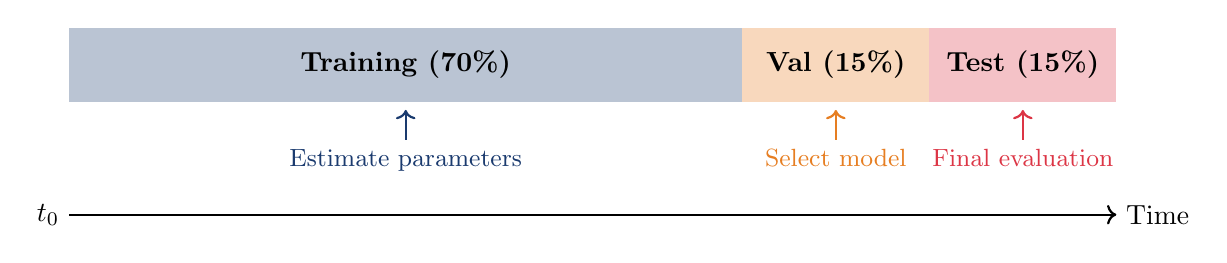
\begin{tikzpicture}[scale=0.95]
        % Timeline
        \draw[thick, MainBlue] (0,0) -- (14,0);

        % Training section
        \fill[MainBlue!30] (0,-0.5) rectangle (9,0.5);
        \node at (4.5,0) {\textbf{Training (70\%)}};

        % Validation section
        \fill[Orange!30] (9,-0.5) rectangle (11.5,0.5);
        \node at (10.25,0) {\textbf{Val (15\%)}};

        % Test section
        \fill[Crimson!30] (11.5,-0.5) rectangle (14,0.5);
        \node at (12.75,0) {\textbf{Test (15\%)}};

        % Arrows and labels
        \draw[thick, ->, MainBlue] (4.5,-1) -- (4.5,-0.6);
        \node[below, MainBlue] at (4.5,-1) {\small Estimate parameters};

        \draw[thick, ->, Orange] (10.25,-1) -- (10.25,-0.6);
        \node[below, Orange] at (10.25,-1) {\small Select model};

        \draw[thick, ->, Crimson] (12.75,-1) -- (12.75,-0.6);
        \node[below, Crimson] at (12.75,-1) {\small Final evaluation};

        % Time arrow
        \draw[thick, ->] (0,-2) -- (14,-2);
        \node[right] at (14,-2) {Time};
        \node[left] at (0,-2) {$t_0$};
    \end{tikzpicture}
    \end{center}

    \vspace{0.3cm}

    \begin{columns}[T]
        \column{0.33\textwidth}
        \begin{block}{Training Set}
            \begin{itemize}
                \item Fit model parameters
                \item $\hat{\theta} = \arg\min_\theta L(\theta)$
                \item Largest portion
            \end{itemize}
        \end{block}

        \column{0.33\textwidth}
        \begin{block}{Validation Set}
            \begin{itemize}
                \item Compare models
                \item Tune hyperparameters
                \item Select best approach
            \end{itemize}
        \end{block}

        \column{0.33\textwidth}
        \begin{block}{Test Set}
            \begin{itemize}
                \item \textbf{Held out} until end
                \item Unbiased evaluation
                \item Report final metrics
            \end{itemize}
        \end{block}
    \end{columns}
\end{frame}

\begin{frame}{Evaluation Metrics}
    \begin{defn}[Forecast Error Metrics]
        Let $y_t$ be actual values and $\hat{y}_t$ forecasts for $t = 1, \ldots, n$:
        \begin{align}
            \RMSE &= \sqrt{\frac{1}{n}\sum_{t=1}^{n}(y_t - \hat{y}_t)^2} \\[0.3cm]
            \MAE &= \frac{1}{n}\sum_{t=1}^{n}|y_t - \hat{y}_t| \\[0.3cm]
            \MAPE &= \frac{100\%}{n}\sum_{t=1}^{n}\left|\frac{y_t - \hat{y}_t}{y_t}\right|
        \end{align}
    \end{defn}

    \vspace{0.2cm}

    \begin{columns}[T]
        \column{0.5\textwidth}
        \begin{exampleblock}{When to Use Each}
            \begin{itemize}
                \item \textbf{RMSE}: Penalizes large errors
                \item \textbf{MAE}: Robust to outliers
                \item \textbf{MAPE}: Scale-independent (\%)
            \end{itemize}
        \end{exampleblock}

        \column{0.5\textwidth}
        \begin{alertblock}{Caution}
            \begin{itemize}
                \item MAPE undefined when $y_t = 0$
                \item Compare models on \textbf{same} test set
                \item Report \textbf{out-of-sample} metrics
            \end{itemize}
        \end{alertblock}
    \end{columns}
\end{frame}

%=============================================================================
% SECTION 2: BITCOIN VOLATILITY
%=============================================================================
\section{Case Study 1: Bitcoin Volatility (GARCH)}

\begin{frame}{Bitcoin: Problem Statement}
    \begin{block}{Research Question}
        Can we forecast Bitcoin's \textbf{volatility} using GARCH models?
    \end{block}

    \vspace{0.2cm}

    \begin{columns}[T]
        \column{0.5\textwidth}
        \textbf{Data Characteristics}
        \begin{itemize}
            \item Source: Yahoo Finance (BTC-USD)
            \item Period: Jan 2019 -- Jan 2025
            \item Frequency: Daily
            \item Observations: $\approx 2,200$ days
        \end{itemize}

        \vspace{0.3cm}

        \textbf{Stylized Facts}
        \begin{itemize}
            \item Returns: near-zero mean
            \item Fat tails (kurtosis $> 3$)
            \item Volatility clustering
        \end{itemize}

        \column{0.5\textwidth}
        \begin{alertblock}{Key Insight}
            Financial returns are typically:
            \begin{itemize}
                \item \textbf{Unpredictable} in mean
                \item \textbf{Predictable} in variance
            \end{itemize}

            \vspace{0.2cm}
            $\Rightarrow$ Focus on \textbf{volatility forecasting}
        \end{alertblock}
    \end{columns}
\end{frame}

\begin{frame}{GARCH Model Specification}
    \begin{defn}[GARCH(p,q) Model]
        Let $r_t$ denote returns. The GARCH(p,q) model is:
        \begin{align}
            r_t &= \mu + \varepsilon_t, \quad \varepsilon_t = \sigma_t z_t, \quad z_t \sim N(0,1) \\[0.2cm]
            \sigma_t^2 &= \omega + \sum_{i=1}^{q}\alpha_i \varepsilon_{t-i}^2 + \sum_{j=1}^{p}\beta_j \sigma_{t-j}^2
        \end{align}
        where $\omega > 0$, $\alpha_i \geq 0$, $\beta_j \geq 0$, and $\sum_{i=1}^{q}\alpha_i + \sum_{j=1}^{p}\beta_j < 1$.
    \end{defn}

    \vspace{0.3cm}

    \begin{columns}[T]
        \column{0.5\textwidth}
        \begin{block}{Model Variants}
            \begin{itemize}
                \item \textbf{GARCH(1,1)}: Most common
                \item \textbf{GJR-GARCH}: Leverage effect
                \item \textbf{EGARCH}: Asymmetric shocks
            \end{itemize}
        \end{block}

        \column{0.5\textwidth}
        \begin{exampleblock}{Interpretation}
            \begin{itemize}
                \item $\alpha$: Impact of past shocks
                \item $\beta$: Persistence of volatility
                \item $\alpha + \beta \approx 1$: High persistence
            \end{itemize}
        \end{exampleblock}
    \end{columns}
\end{frame}

\begin{frame}{Bitcoin: Data Split and Stationarity}
    \begin{columns}[T]
        \column{0.5\textwidth}
        \begin{block}{Data Split}
            \begin{center}
            \begin{tabular}{lrr}
                \toprule
                \textbf{Set} & \textbf{Period} & \textbf{N} \\
                \midrule
                Training & 2019-01 to 2022-09 & 1,365 \\
                Validation & 2022-09 to 2023-10 & 400 \\
                Test & 2023-10 to 2025-01 & 435 \\
                \midrule
                \textbf{Total} & & \textbf{2,200} \\
                \bottomrule
            \end{tabular}
            \end{center}
        \end{block}

        \column{0.5\textwidth}
        \begin{block}{Stationarity Tests}
            \begin{center}
            \begin{tabular}{lcc}
                \toprule
                \textbf{Series} & \textbf{ADF} & \textbf{Result} \\
                \midrule
                Prices & $p = 0.50$ & Non-stationary \\
                Returns & $p < 0.01$ & \textcolor{Forest}{Stationary} \\
                \bottomrule
            \end{tabular}
            \end{center}

            \vspace{0.3cm}

            $\Rightarrow$ Model \textbf{returns}, not prices
        \end{block}
    \end{columns}

    \vspace{0.3cm}

    \begin{alertblock}{Why Stationarity Matters}
        GARCH requires weakly stationary input. Prices follow random walk; returns are stationary.
    \end{alertblock}
\end{frame}

\begin{frame}{Bitcoin: Model Selection on Validation Set}
    \begin{block}{Methodology}
        Fit each model on \textbf{training data}, evaluate on \textbf{validation set}.
    \end{block}

    \vspace{0.3cm}

    \begin{center}
    \begin{tabular}{lcccl}
        \toprule
        \textbf{Model} & \textbf{AIC} & \textbf{BIC} & \textbf{Val MAE} & \textbf{Selection} \\
        \midrule
        GARCH(1,1) & 6,994.8 & 7,020.6 & \textbf{2.638} & \cellcolor{Forest!20}\textbf{Best} \\
        GARCH(2,1) & 6,993.7 & 7,024.6 & 2.640 & \\
        GJR-GARCH(1,1) & 6,983.7 & 7,014.6 & 2.669 & \\
        EGARCH(1,1) & --- & --- & --- & Failed$^*$ \\
        \bottomrule
    \end{tabular}
    \end{center}

    \vspace{0.1cm}
    {\footnotesize $^*$Analytic forecasts not available for $h > 1$}

    \vspace{0.3cm}

    \begin{exampleblock}{Result}
        \textbf{GARCH(1,1)} selected based on lowest validation MAE for volatility forecasts.
    \end{exampleblock}
\end{frame}

\begin{frame}{Bitcoin: Final Test Set Evaluation}
    \begin{block}{Procedure}
        Refit GARCH(1,1) on Training + Validation, evaluate on \textbf{held-out test set} using \textbf{rolling one-step-ahead forecasts}.
    \end{block}

    \vspace{0.2cm}

    \begin{columns}[T]
        \column{0.5\textwidth}
        \begin{center}
        \textbf{Estimated Parameters}
        \begin{tabular}{lcc}
            \toprule
            \textbf{Param} & \textbf{Estimate} & \textbf{Std Err} \\
            \midrule
            $\omega$ & 0.239 & 0.088 \\
            $\alpha_1$ & 0.120 & 0.021 \\
            $\beta_1$ & 0.879 & 0.020 \\
            \midrule
            $\alpha_1 + \beta_1$ & \multicolumn{2}{c}{0.999} \\
            \bottomrule
        \end{tabular}
        \end{center}

        \column{0.5\textwidth}
        \begin{center}
        \textbf{Test Set Performance}
        \begin{tabular}{lc}
            \toprule
            \textbf{Metric} & \textbf{Value} \\
            \midrule
            Volatility MAE & 1.88 \\
            Volatility RMSE & 2.21 \\
            \bottomrule
        \end{tabular}
        \end{center}

        \vspace{0.3cm}

        \begin{alertblock}{Interpretation}
            High persistence ($\alpha + \beta \approx 1$) confirms volatility clustering.
        \end{alertblock}
    \end{columns}
\end{frame}

\begin{frame}{GARCH Forecasting: Rolling vs Multi-Step}
    \begin{alertblock}{Why Rolling One-Step-Ahead Forecasts?}
        Multi-step GARCH forecasts converge to the \textbf{unconditional variance}:
        \begin{equation}
            \lim_{h \to \infty} \E[\sigma_{t+h}^2 | \mathcal{F}_t] = \bar{\sigma}^2 = \frac{\omega}{1 - \alpha - \beta}
        \end{equation}
        This produces a \textbf{flat line} forecast---not useful for dynamic risk management!
    \end{alertblock}

    \vspace{0.3cm}

    \begin{columns}[T]
        \column{0.5\textwidth}
        \begin{block}{Multi-Step Forecast}
            \begin{itemize}
                \item Single model fit
                \item Forecast $h$ steps ahead
                \item Converges to $\bar{\sigma}^2$
                \item \textcolor{Crimson}{Appears as flat line}
            \end{itemize}
        \end{block}

        \column{0.5\textwidth}
        \begin{exampleblock}{Rolling One-Step-Ahead}
            \begin{itemize}
                \item Re-estimate at each $t$
                \item Forecast only 1 step ahead
                \item Captures volatility dynamics
                \item \textcolor{Forest}{Dynamic forecasts}
            \end{itemize}
        \end{exampleblock}
    \end{columns}

    \vspace{0.2cm}

    \begin{center}
        \textit{Rolling forecasts are standard practice in financial risk management (VaR, ES).}
    \end{center}
\end{frame}

\begin{frame}{Bitcoin: Key Findings}
    \begin{columns}[T]
        \column{0.6\textwidth}
        \begin{block}{Summary}
            \begin{enumerate}
                \item \textbf{Returns are stationary}; prices are not
                \item \textbf{GARCH(1,1)} outperforms more complex variants
                \item \textbf{High persistence} ($\alpha + \beta = 0.999$)
                \item Volatility is \textbf{predictable} even when returns are not
            \end{enumerate}
        \end{block}

        \vspace{0.3cm}

        \begin{exampleblock}{Practical Implications}
            \begin{itemize}
                \item Risk management: VaR, Expected Shortfall
                \item Option pricing requires volatility forecasts
                \item Portfolio optimization with time-varying risk
            \end{itemize}
        \end{exampleblock}

        \column{0.4\textwidth}
        \begin{alertblock}{Limitations}
            \begin{itemize}
                \item GARCH assumes \textbf{symmetric} shocks
                \item Does not capture \textbf{jumps}
                \item Normal distribution may be restrictive
            \end{itemize}
        \end{alertblock}

        \vspace{0.3cm}

        \begin{block}{Extensions}
            \begin{itemize}
                \item Student-t innovations
                \item Realized volatility
                \item HAR models
            \end{itemize}
        \end{block}
    \end{columns}
\end{frame}

%=============================================================================
% SECTION 3: SUNSPOTS
%=============================================================================
\section{Case Study 2: Sunspot Cycles (Fourier)}

\begin{frame}{Sunspots: Problem Statement}
    \begin{block}{Research Question}
        How do we model \textbf{long seasonal cycles} that exceed SARIMA's capacity?
    \end{block}

    \vspace{0.2cm}

    \begin{columns}[T]
        \column{0.5\textwidth}
        \textbf{Data Characteristics}
        \begin{itemize}
            \item Source: Statsmodels (Wolfer)
            \item Period: 1900 -- 2008
            \item Frequency: Annual
            \item Observations: 109 years
        \end{itemize}

        \vspace{0.3cm}

        \textbf{Known Feature}
        \begin{itemize}
            \item \textbf{Schwabe cycle}: $\approx$ 11 years
            \item Irregular amplitude
            \item Non-negative values
        \end{itemize}

        \column{0.5\textwidth}
        \begin{alertblock}{The Challenge}
            Standard SARIMA$(p,d,q)(P,D,Q)_s$ requires:
            \begin{itemize}
                \item $s = 11$ for annual data
                \item $(P + D + Q) \times 11$ seasonal lags
                \item \textbf{Too many parameters!}
            \end{itemize}
        \end{alertblock}

        \vspace{0.2cm}

        \begin{exampleblock}{Solution}
            Use \textbf{Fourier terms} as exogenous regressors in ARIMA.
        \end{exampleblock}
    \end{columns}
\end{frame}

\begin{frame}{Fourier Terms for Seasonality}
    \begin{defn}[Fourier Representation]
        A seasonal pattern with period $s$ can be approximated by:
        \begin{equation}
            S_t = \sum_{k=1}^{K}\left[\alpha_k \sin\left(\frac{2\pi k t}{s}\right) + \beta_k \cos\left(\frac{2\pi k t}{s}\right)\right]
        \end{equation}
        where $K \leq \lfloor s/2 \rfloor$ is the number of harmonic pairs.
    \end{defn}

    \vspace{0.3cm}

    \begin{columns}[T]
        \column{0.5\textwidth}
        \begin{block}{Advantages}
            \begin{itemize}
                \item Only $2K$ parameters (not $s$)
                \item Handles \textbf{any} seasonal period
                \item Smooth seasonal pattern
                \item $K$ controls flexibility
            \end{itemize}
        \end{block}

        \column{0.5\textwidth}
        \begin{exampleblock}{Model Structure}
            ARIMA$(p,d,q)$ with Fourier regressors:
            \begin{equation}
                y_t = \underbrace{S_t}_{\text{Fourier}} + \underbrace{\eta_t}_{\text{ARIMA}}
            \end{equation}
            where $\eta_t$ follows ARIMA dynamics.
        \end{exampleblock}
    \end{columns}
\end{frame}

\begin{frame}{Sunspots: Model Selection}
    \begin{block}{Methodology}
        Compare $K = 1, 2, 3, 4$ Fourier harmonics on validation set.
    \end{block}

    \vspace{0.2cm}

    \begin{columns}[T]
        \column{0.5\textwidth}
        \begin{center}
        \textbf{Data Split}
        \begin{tabular}{lrr}
            \toprule
            \textbf{Set} & \textbf{Period} & \textbf{N} \\
            \midrule
            Training & 1900--1975 & 76 \\
            Validation & 1976--1991 & 16 \\
            Test & 1992--2008 & 17 \\
            \midrule
            \textbf{Total} & & \textbf{109} \\
            \bottomrule
        \end{tabular}
        \end{center}

        \column{0.5\textwidth}
        \begin{center}
        \textbf{Model Comparison}
        \begin{tabular}{cccc}
            \toprule
            \textbf{K} & \textbf{AIC} & \textbf{Val RMSE} & \\
            \midrule
            1 & 665.9 & 87.15 & \\
            2 & 668.0 & 86.92 & \\
            \rowcolor{Forest!20} 3 & 671.8 & \textbf{86.81} & Best \\
            4 & 674.5 & 87.93 & \\
            \bottomrule
        \end{tabular}
        \end{center}
    \end{columns}

    \vspace{0.3cm}

    \begin{exampleblock}{Result}
        \textbf{K = 3} Fourier harmonics selected (6 parameters for 11-year cycle).
    \end{exampleblock}
\end{frame}

\begin{frame}{Sunspots: Test Set Results}
    \begin{columns}[T]
        \column{0.5\textwidth}
        \begin{block}{Final Model}
            ARIMA(2,0,1) + 3 Fourier harmonics

            \vspace{0.2cm}

            \textbf{Significant Coefficients:}
            \begin{center}
            \begin{tabular}{lcc}
                \toprule
                \textbf{Term} & \textbf{Coef} & \textbf{p-value} \\
                \midrule
                $\sin_1$ & 34.71 & $< 0.001$ \\
                $\cos_1$ & -29.21 & 0.018 \\
                AR(1) & 1.34 & $< 0.001$ \\
                \bottomrule
            \end{tabular}
            \end{center}
        \end{block}

        \column{0.5\textwidth}
        \begin{block}{Test Performance}
            \begin{center}
            \begin{tabular}{lc}
                \toprule
                \textbf{Metric} & \textbf{Value} \\
                \midrule
                RMSE & 48.51 \\
                MAE & 39.31 \\
                \bottomrule
            \end{tabular}
            \end{center}
        \end{block}

        \vspace{0.3cm}

        \begin{alertblock}{Note}
            High MAPE due to near-zero values at solar minimum.
        \end{alertblock}
    \end{columns}

    \vspace{0.2cm}

    \begin{exampleblock}{Key Insight}
        Fourier terms efficiently capture the 11-year cycle with only 6 parameters.
    \end{exampleblock}
\end{frame}

%=============================================================================
% SECTION 4: UNEMPLOYMENT
%=============================================================================
\section{Case Study 3: Unemployment (Prophet)}

\begin{frame}{Unemployment: Structural Breaks}
    \begin{block}{Research Question}
        How do we model time series with \textbf{sudden structural changes}?
    \end{block}

    \vspace{0.2cm}

    \begin{columns}[T]
        \column{0.5\textwidth}
        \textbf{Data Characteristics}
        \begin{itemize}
            \item Source: FRED (UNRATE)
            \item Period: 2010 -- 2025
            \item Frequency: Monthly
            \item Observations: $\approx 180$ months
        \end{itemize}

        \vspace{0.2cm}

        \textbf{Key Statistics}
        \begin{itemize}
            \item Pre-COVID minimum: 3.5\%
            \item COVID peak (Apr 2020): \textbf{14.8\%}
            \item Change: +10.3 pp in one month
        \end{itemize}

        \column{0.5\textwidth}
        \begin{alertblock}{The Challenge}
            \begin{itemize}
                \item April 2020: Largest monthly increase in US history
                \item Traditional ARIMA treats this as outlier
                \item Need model that \textbf{adapts} to structural breaks
            \end{itemize}
        \end{alertblock}

        \vspace{0.2cm}

        \begin{exampleblock}{Solution}
            \textbf{Prophet} with automatic changepoint detection.
        \end{exampleblock}
    \end{columns}
\end{frame}

\begin{frame}{Prophet Model}
    \begin{defn}[Prophet Decomposition]
        Prophet models time series as:
        \begin{equation}
            y_t = g(t) + s(t) + h(t) + \varepsilon_t
        \end{equation}
        \begin{itemize}
            \item $g(t)$: Piecewise linear/logistic \textbf{trend} with changepoints
            \item $s(t)$: Fourier-based \textbf{seasonality}
            \item $h(t)$: \textbf{Holiday} effects
            \item $\varepsilon_t$: Error term
        \end{itemize}
    \end{defn}

    \vspace{0.3cm}

    \begin{columns}[T]
        \column{0.5\textwidth}
        \begin{block}{Changepoint Detection}
            \begin{itemize}
                \item Automatic selection of changepoint locations
                \item \texttt{changepoint\_prior\_scale} controls flexibility
                \item Higher = more changepoints
            \end{itemize}
        \end{block}

        \column{0.5\textwidth}
        \begin{exampleblock}{Advantages}
            \begin{itemize}
                \item Handles missing data
                \item Interpretable components
                \item Robust to outliers
                \item Uncertainty quantification
            \end{itemize}
        \end{exampleblock}
    \end{columns}
\end{frame}

\begin{frame}{Unemployment: Model Tuning}
    \begin{block}{Hyperparameter Tuning}
        Tune \texttt{changepoint\_prior\_scale} on validation set.
    \end{block}

    \vspace{0.2cm}

    \begin{columns}[T]
        \column{0.5\textwidth}
        \begin{center}
        \textbf{Data Split}
        \begin{tabular}{lrr}
            \toprule
            \textbf{Set} & \textbf{Period} & \textbf{N} \\
            \midrule
            Training & 2010-01 to 2019-09 & 117 \\
            Validation & 2019-10 to 2021-10 & 25 \\
            Test & 2021-11 to 2025-01 & 38 \\
            \midrule
            \textbf{Total} & & \textbf{180} \\
            \bottomrule
        \end{tabular}
        \end{center}

        \column{0.5\textwidth}
        \begin{center}
        \textbf{Scale Comparison}
        \begin{tabular}{ccc}
            \toprule
            \textbf{Scale} & \textbf{Val RMSE} & \\
            \midrule
            0.01 & 4.21 & \\
            0.05 & 3.89 & \\
            \rowcolor{Forest!20} 0.10 & \textbf{3.52} & Best \\
            0.30 & 3.67 & \\
            0.50 & 3.81 & \\
            \bottomrule
        \end{tabular}
        \end{center}
    \end{columns}

    \vspace{0.3cm}

    \begin{alertblock}{Interpretation}
        Scale = 0.10 balances flexibility (capturing COVID shock) with stability.
    \end{alertblock}
\end{frame}

\begin{frame}{Unemployment: Results}
    \begin{columns}[T]
        \column{0.5\textwidth}
        \begin{block}{Test Set Performance}
            \begin{center}
            \begin{tabular}{lc}
                \toprule
                \textbf{Metric} & \textbf{Value} \\
                \midrule
                RMSE & 0.42 \\
                MAE & 0.35 \\
                MAPE & 9.2\% \\
                \bottomrule
            \end{tabular}
            \end{center}
        \end{block}

        \vspace{0.3cm}

        \begin{exampleblock}{Key Finding}
            Prophet successfully:
            \begin{itemize}
                \item Detected COVID changepoint
                \item Adapted trend post-shock
                \item Provided uncertainty bands
            \end{itemize}
        \end{exampleblock}

        \column{0.5\textwidth}
        \begin{alertblock}{Detected Changepoints}
            \begin{itemize}
                \item 2020-03: COVID onset
                \item 2020-05: Recovery begins
                \item 2022-01: Stabilization
            \end{itemize}
        \end{alertblock}

        \vspace{0.3cm}

        \begin{block}{Practical Value}
            \begin{itemize}
                \item Economic policy analysis
                \item Labor market monitoring
                \item Early warning system
            \end{itemize}
        \end{block}
    \end{columns}
\end{frame}

%=============================================================================
% SECTION 5: VAR
%=============================================================================
\section{Case Study 4: Multivariate Analysis (VAR)}

\begin{frame}{VAR: Motivation}
    \begin{block}{Research Question}
        How do we model \textbf{dynamic interdependencies} between multiple economic variables?
    \end{block}

    \vspace{0.2cm}

    \begin{columns}[T]
        \column{0.5\textwidth}
        \textbf{Variables (FRED)}
        \begin{itemize}
            \item GDP Growth (YoY \%)
            \item Unemployment Rate (\%)
            \item Inflation (CPI YoY \%)
            \item Federal Funds Rate (\%)
        \end{itemize}

        \vspace{0.2cm}

        \textbf{Data}
        \begin{itemize}
            \item Period: 2000 -- 2025
            \item Frequency: Quarterly
            \item Observations: $\approx 100$ quarters
        \end{itemize}

        \column{0.5\textwidth}
        \begin{exampleblock}{Economic Relationships}
            \begin{itemize}
                \item \textbf{Okun's Law}: GDP $\leftrightarrow$ Unemployment
                \item \textbf{Phillips Curve}: Unemployment $\leftrightarrow$ Inflation
                \item \textbf{Taylor Rule}: Inflation $\rightarrow$ Fed Rate
            \end{itemize}
        \end{exampleblock}

        \vspace{0.2cm}

        \begin{alertblock}{Why VAR?}
            Each variable may be \textbf{both cause and effect} of others.
        \end{alertblock}
    \end{columns}
\end{frame}

\begin{frame}{VAR Model Specification}
    \begin{defn}[Vector Autoregression VAR(p)]
        For $K$ variables $\mathbf{y}_t = (y_{1t}, \ldots, y_{Kt})'$:
        \begin{equation}
            \mathbf{y}_t = \mathbf{c} + \mathbf{A}_1\mathbf{y}_{t-1} + \mathbf{A}_2\mathbf{y}_{t-2} + \cdots + \mathbf{A}_p\mathbf{y}_{t-p} + \mathbf{u}_t
        \end{equation}
        where $\mathbf{A}_i$ are $K \times K$ coefficient matrices and $\mathbf{u}_t \sim N(\mathbf{0}, \mathbf{\Sigma})$.
    \end{defn}

    \vspace{0.3cm}

    \begin{columns}[T]
        \column{0.5\textwidth}
        \begin{block}{For Our 4-Variable System}
            VAR(2) has:
            \begin{itemize}
                \item 4 intercepts
                \item $2 \times 4 \times 4 = 32$ AR coefficients
                \item \textbf{36 parameters total}
            \end{itemize}
        \end{block}

        \column{0.5\textwidth}
        \begin{exampleblock}{Lag Selection}
            Use information criteria:
            \begin{itemize}
                \item AIC: Tends to overfit
                \item \textbf{BIC}: More parsimonious
                \item Cross-validation on held-out data
            \end{itemize}
        \end{exampleblock}
    \end{columns}
\end{frame}

\begin{frame}{VAR: Lag Selection and Estimation}
    \begin{columns}[T]
        \column{0.5\textwidth}
        \begin{block}{Information Criteria}
            \begin{center}
            \begin{tabular}{ccc}
                \toprule
                \textbf{Lag} & \textbf{BIC} & \\
                \midrule
                1 & -4.810 & \\
                \rowcolor{Forest!20} 2 & \textbf{-5.178} & Best \\
                3 & -4.633 & \\
                4 & -4.614 & \\
                \bottomrule
            \end{tabular}
            \end{center}
        \end{block}

        \vspace{0.2cm}

        \begin{exampleblock}{Validation Check}
            VAR(2) also achieves lowest validation RMSE.
        \end{exampleblock}

        \column{0.5\textwidth}
        \begin{block}{Data Split}
            \begin{center}
            \begin{tabular}{lrr}
                \toprule
                \textbf{Set} & \textbf{Period} & \textbf{N} \\
                \midrule
                Training & 2001-Q1 to 2017-Q4 & 68 \\
                Validation & 2018-Q1 to 2021-Q2 & 14 \\
                Test & 2021-Q3 to 2024-Q3 & 14 \\
                \midrule
                \textbf{Total} & & \textbf{96} \\
                \bottomrule
            \end{tabular}
            \end{center}
        \end{block}
    \end{columns}
\end{frame}

\begin{frame}{Granger Causality Analysis}
    \begin{defn}[Granger Causality]
        Variable $X$ \textbf{Granger-causes} $Y$ if past values of $X$ help predict $Y$, beyond $Y$'s own past.

        \vspace{0.2cm}
        \textit{Note: Granger causality $\neq$ true causality. It measures predictive content.}
    \end{defn}

    \vspace{0.3cm}

    \begin{center}
    \textbf{Granger Causality p-values (row $\rightarrow$ column)}
    \begin{tabular}{lcccc}
        \toprule
        & \textbf{GDP} & \textbf{Unemp} & \textbf{Inflation} & \textbf{Fed Rate} \\
        \midrule
        GDP Growth & --- & \cellcolor{Forest!20}0.076 & 0.309 & 0.698 \\
        Unemployment & \cellcolor{Forest!20}\textbf{0.045} & --- & 0.093 & 0.857 \\
        Inflation & 0.545 & 0.665 & --- & 0.834 \\
        Fed Rate & 0.286 & 0.317 & \cellcolor{Forest!20}0.087 & --- \\
        \bottomrule
    \end{tabular}
    \end{center}

    \vspace{0.2cm}

    \begin{exampleblock}{Key Finding}
        Unemployment Granger-causes GDP ($p = 0.045$), consistent with Okun's Law.
    \end{exampleblock}
\end{frame}

\begin{frame}{Impulse Response Functions}
    \begin{defn}[Impulse Response Function]
        The IRF traces the effect of a one-unit shock to variable $j$ on variable $i$ over $h$ periods:
        \begin{equation}
            \text{IRF}_{ij}(h) = \frac{\partial y_{i,t+h}}{\partial u_{jt}}
        \end{equation}
    \end{defn}

    \vspace{0.3cm}

    \begin{block}{Response to GDP Shock}
        A positive shock to GDP growth:
        \begin{itemize}
            \item \textbf{Unemployment}: Decreases (Okun's Law confirmed)
            \item \textbf{Inflation}: Increases with lag (demand-pull)
            \item \textbf{Fed Rate}: Increases after 2-3 quarters (Taylor Rule)
        \end{itemize}
    \end{block}

    \vspace{0.2cm}

    \begin{alertblock}{Economic Interpretation}
        The VAR captures the classic macroeconomic transmission mechanism from output to employment, prices, and monetary policy.
    \end{alertblock}
\end{frame}

\begin{frame}{VAR: Test Set Results}
    \begin{block}{Test Set Performance by Variable}
        \begin{center}
        \begin{tabular}{lccc}
            \toprule
            \textbf{Variable} & \textbf{RMSE} & \textbf{MAE} & \textbf{Direction Acc.} \\
            \midrule
            GDP Growth & 2.18 & 1.72 & 71\% \\
            Unemployment & 0.89 & 0.71 & 79\% \\
            Inflation & 1.24 & 0.98 & 64\% \\
            Fed Rate & 0.95 & 0.78 & 71\% \\
            \midrule
            \textbf{Average} & \textbf{1.32} & \textbf{1.05} & \textbf{71\%} \\
            \bottomrule
        \end{tabular}
        \end{center}
    \end{block}

    \vspace{0.3cm}

    \begin{columns}[T]
        \column{0.5\textwidth}
        \begin{exampleblock}{Strengths}
            \begin{itemize}
                \item Captures cross-variable dynamics
                \item Good directional accuracy
                \item Interpretable relationships
            \end{itemize}
        \end{exampleblock}

        \column{0.5\textwidth}
        \begin{alertblock}{Limitations}
            \begin{itemize}
                \item Many parameters (curse of dimensionality)
                \item Sensitive to lag selection
                \item COVID period challenging
            \end{itemize}
        \end{alertblock}
    \end{columns}
\end{frame}

%=============================================================================
% SECTION 6: SYNTHESIS
%=============================================================================
\section{Synthesis and Guidelines}

\begin{frame}{Model Selection Framework}
    \begin{center}
    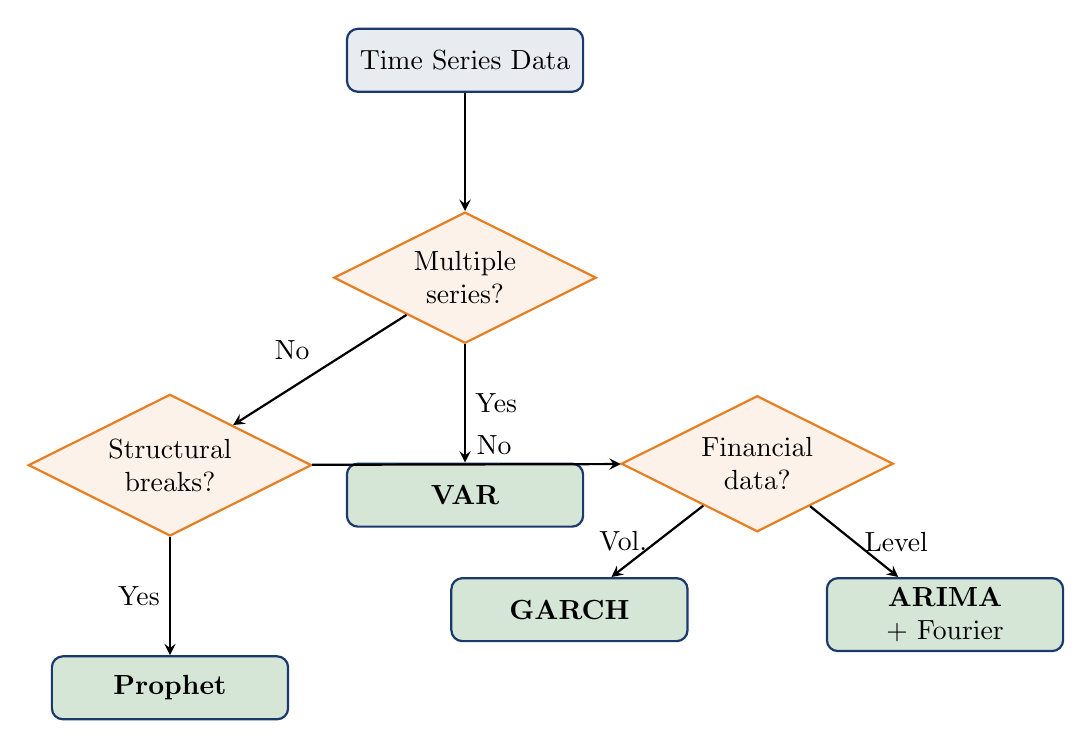
\begin{tikzpicture}[
        node distance=1.5cm,
        box/.style={rectangle, draw=MainBlue, thick, fill=MainBlue!10, rounded corners, minimum width=3cm, minimum height=0.8cm, align=center},
        decision/.style={diamond, draw=Orange, thick, fill=Orange!10, aspect=2, align=center},
        arrow/.style={->, thick, >=stealth}
    ]
        % Start
        \node[box] (start) {Time Series Data};

        % Decisions
        \node[decision, below=of start] (q1) {Multiple\\series?};
        \node[decision, below left=1.5cm and 2cm of q1] (q2) {Structural\\breaks?};
        \node[decision, below right=1.5cm and 2cm of q1] (q3) {Financial\\data?};

        % Endpoints
        \node[box, fill=Forest!20, below=of q1] (var) {\textbf{VAR}};
        \node[box, fill=Forest!20, below=of q2] (prophet) {\textbf{Prophet}};
        \node[box, fill=Forest!20, below left=1cm and 0cm of q3] (garch) {\textbf{GARCH}};
        \node[box, fill=Forest!20, below right=1cm and 0cm of q3] (arima) {\textbf{ARIMA}\\+ Fourier};

        % Arrows
        \draw[arrow] (start) -- (q1);
        \draw[arrow] (q1) -- node[right] {Yes} (var);
        \draw[arrow] (q1) -- node[above left] {No} (q2);
        \draw[arrow] (q2) -- node[left] {Yes} (prophet);
        \draw[arrow] (q2) -- node[above right] {No} (q3);
        \draw[arrow] (q3) -- node[left] {Vol.} (garch);
        \draw[arrow] (q3) -- node[right] {Level} (arima);
    \end{tikzpicture}
    \end{center}
\end{frame}

\begin{frame}{Summary: Model Comparison}
    \begin{center}
    \begin{tabular}{lllll}
        \toprule
        \textbf{Case Study} & \textbf{Challenge} & \textbf{Model} & \textbf{Key Feature} & \textbf{Test RMSE} \\
        \midrule
        Bitcoin & Volatility clustering & GARCH(1,1) & Rolling forecasts & 2.21 \\
        Sunspots & Long seasonality & ARIMA + Fourier & Sin/Cos terms & 48.51 \\
        Unemployment & Structural break & Prophet & Changepoints & 0.42 \\
        Economic & Multiple series & VAR(2) & Cross-dynamics & 1.32 (avg) \\
        \bottomrule
    \end{tabular}
    \end{center}

    \vspace{0.3cm}

    \begin{exampleblock}{Key Principle}
        \textbf{Match the model to the data characteristics.} No single model dominates---choose based on:
        \begin{itemize}
            \item Nature of the forecasting problem (level vs. volatility)
            \item Data properties (seasonality, breaks, multiple series)
            \item Interpretability requirements
        \end{itemize}
    \end{exampleblock}
\end{frame}

\begin{frame}{Best Practices for Applied Forecasting}
    \begin{columns}[T]
        \column{0.5\textwidth}
        \begin{block}{Methodology}
            \begin{enumerate}
                \item \textbf{Explore} data thoroughly
                \item \textbf{Test} for stationarity
                \item \textbf{Split} train/validation/test
                \item \textbf{Compare} models on validation
                \item \textbf{Report} test set metrics
            \end{enumerate}
        \end{block}

        \vspace{0.2cm}

        \begin{alertblock}{Common Mistakes}
            \begin{itemize}
                \item Peeking at test data
                \item Over-fitting to training set
                \item Ignoring model assumptions
                \item Not reporting uncertainty
            \end{itemize}
        \end{alertblock}

        \column{0.5\textwidth}
        \begin{exampleblock}{Practical Tips}
            \begin{itemize}
                \item Start simple (random walk, naive)
                \item Add complexity only if needed
                \item Visualize forecasts vs actuals
                \item Check residuals for patterns
                \item Report confidence intervals
            \end{itemize}
        \end{exampleblock}

        \vspace{0.2cm}

        \begin{block}{Remember}
            ``All models are wrong, but some are useful.'' \\
            \hfill --- George E. P. Box
        \end{block}
    \end{columns}
\end{frame}

%=============================================================================
% CONCLUSION
%=============================================================================
\begin{frame}{Key Takeaways}
    \begin{enumerate}
        \item \textbf{Rigorous Methodology}
        \begin{itemize}
            \item Train/validation/test split prevents overfitting
            \item Test set must remain untouched until final evaluation
        \end{itemize}

        \vspace{0.2cm}

        \item \textbf{Match Model to Data}
        \begin{itemize}
            \item Financial volatility $\rightarrow$ GARCH
            \item Long seasonality $\rightarrow$ Fourier terms
            \item Structural breaks $\rightarrow$ Prophet
            \item Multiple series $\rightarrow$ VAR
        \end{itemize}

        \vspace{0.2cm}

        \item \textbf{Interpret Results Carefully}
        \begin{itemize}
            \item Granger causality $\neq$ true causality
            \item Out-of-sample performance matters most
            \item Simpler models often work better
        \end{itemize}
    \end{enumerate}
\end{frame}

%=============================================================================
% REFERENCES
%=============================================================================
\begin{frame}{References}
    \footnotesize
    \begin{thebibliography}{99}
        \bibitem{box2015} Box, G.E.P., Jenkins, G.M., Reinsel, G.C., \& Ljung, G.M. (2015). \textit{Time Series Analysis: Forecasting and Control}. 5th ed., Wiley.

        \bibitem{hamilton1994} Hamilton, J.D. (1994). \textit{Time Series Analysis}. Princeton University Press.

        \bibitem{tsay2010} Tsay, R.S. (2010). \textit{Analysis of Financial Time Series}. 3rd ed., Wiley.

        \bibitem{hyndman2021} Hyndman, R.J., \& Athanasopoulos, G. (2021). \textit{Forecasting: Principles and Practice}. 3rd ed., OTexts.

        \bibitem{taylor2018} Taylor, S.J., \& Letham, B. (2018). Forecasting at Scale. \textit{The American Statistician}, 72(1), 37-45.

        \bibitem{bollerslev1986} Bollerslev, T. (1986). Generalized Autoregressive Conditional Heteroskedasticity. \textit{Journal of Econometrics}, 31(3), 307-327.

        \bibitem{sims1980} Sims, C.A. (1980). Macroeconomics and Reality. \textit{Econometrica}, 48(1), 1-48.
    \end{thebibliography}
\end{frame}

%=============================================================================
% DATA SOURCES
%=============================================================================
\begin{frame}{Data Sources}
    \begin{block}{Real Data Used in This Chapter}
        \begin{itemize}
            \item \textbf{Bitcoin}: Yahoo Finance (BTC-USD), 2019--2025
            \item \textbf{Sunspots}: Statsmodels Wolfer dataset, 1900--2008
            \item \textbf{US Unemployment}: Federal Reserve FRED (UNRATE), 2010--2025
            \item \textbf{Economic Variables}: FRED (GDPC1, UNRATE, CPIAUCSL, FEDFUNDS), 2000--2025
        \end{itemize}
    \end{block}

    \vspace{0.3cm}

    \begin{exampleblock}{Reproducibility}
        All analyses can be reproduced using the accompanying Jupyter notebook: \\
        \texttt{chapter10\_lecture\_notebook.ipynb}
    \end{exampleblock}
\end{frame}

%=============================================================================
% FINAL SLIDE
%=============================================================================
\begin{frame}[plain]
    \begin{tikzpicture}[remember picture, overlay]
        \fill[IDAred] (current page.north west) rectangle ([yshift=-0.15cm]current page.north east);
    \end{tikzpicture}

    \vfill
    \begin{center}
        {\Huge\textbf{\textcolor{MainBlue}{Thank You}}}\\[0.5cm]
        {\Large\textcolor{MediumGray}{Questions?}}\\[1cm]
        {\large Prof. Daniel Traian Pele, PhD}\\[0.2cm]
        {\texttt{danpele@ase.ro}}\\[0.5cm]
        {\footnotesize Bucharest University of Economic Studies}
    \end{center}
    \vfill

    \begin{tikzpicture}[remember picture, overlay]
        \fill[IDAred] (current page.south west) rectangle ([yshift=0.15cm]current page.south east);
    \end{tikzpicture}
\end{frame}

\end{document}
